\documentclass[11pt]{article}
\usepackage[a4paper,margin=26mm,headheight=14pt]{geometry}
\usepackage[T1]{fontenc}
\usepackage{lmodern,microtype}
\usepackage{amsmath,amssymb,amsthm,mathtools}
\usepackage{booktabs,longtable,tabularx,array}
\usepackage{xcolor,graphicx,enumitem,fancyhdr,listings}
\usepackage{xurl}
\usepackage[colorlinks=true,linkcolor=teal!60!black,citecolor=teal!60!black,urlcolor=blue!50!black]{hyperref}
\definecolor{ink}{HTML}{163348}
\definecolor{accent}{HTML}{007F82}
\definecolor{light}{HTML}{EEF5F5}
\hypersetup{pdftitle={Beyond Dirichlet GRH: sharp torsion selection and tensor detectors},
 pdfauthor={Research report prepared for Vladimir Reshetnikov},
 pdfsubject={Source analysis, exact torsion minimax, and nonabelian transfer criteria}}
\setlength{\parskip}{5pt}
\setlength{\parindent}{0pt}
\setlength{\emergencystretch}{2em}
\setlist{itemsep=3pt,topsep=4pt}
\pagestyle{fancy}
\fancyhf{}
\fancyhead[L]{\small\textcolor{ink}{Beyond Dirichlet GRH}}
\fancyhead[R]{\small 25 November 2026}
\fancyfoot[C]{\thepage}
\renewcommand{\headrulewidth}{0.3pt}
\newtheorem{theorem}{Theorem}[section]
\newtheorem{proposition}[theorem]{Proposition}
\newtheorem{lemma}[theorem]{Lemma}
\newtheorem{corollary}[theorem]{Corollary}
\theoremstyle{definition}
\newtheorem{definition}[theorem]{Definition}
\newtheorem{example}[theorem]{Example}
\theoremstyle{remark}
\newtheorem{remark}[theorem]{Remark}
\newcommand{\Cp}{\mathbf C_p}
\newcommand{\Qp}{\mathbf Q_p}
\newcommand{\Zp}{\mathbf Z_p}
\newcommand{\Ocal}{\mathcal O}
\newcommand{\Gcal}{\mathcal G}
\newcommand{\Reg}{\operatorname{Reg}}
\newcommand{\ord}{\operatorname{ord}}
\newcommand{\Ind}{\operatorname{Ind}}
\newcommand{\Res}{\operatorname{Res}}
\newcommand{\Gal}{\operatorname{Gal}}
\newcommand{\Tr}{\operatorname{Tr}}
\newcommand{\Rea}{\operatorname{Re}}
\newcommand{\Frob}{\operatorname{Frob}}
\newcommand{\one}{\mathbf 1}
\newcommand{\floor}[1]{\left\lfloor #1\right\rfloor}
\newcommand{\ceil}[1]{\left\lceil #1\right\rceil}
\newcommand{\src}[2]{\href{https://github.com/lsernau/grh-lean/blob/72fead102f663d5c7a407964a13dc0cf9d977207/grh/src/#1}{#2}}
\newcommand{\prior}[2]{\href{https://github.com/VladimirReshetnikov/ProveIt/blob/274841c1cb137aafbb60ab5f519c51fd42eee98e/docs/incoming/#1}{#2}}
\lstset{basicstyle=\ttfamily\footnotesize,breaklines=true,columns=fullflexible,
 frame=single,rulecolor=\color{light},backgroundcolor=\color{light},
 keepspaces=true,showstringspaces=false}
\begin{document}
\hypersetup{pageanchor=false}
\begin{titlepage}
\vspace*{14mm}
{\color{accent}\large RESEARCH REPORT\par}
\vspace{7mm}
{\color{ink}\Huge\bfseries Beyond Dirichlet GRH\par}
\vspace{5mm}
{\color{ink}\LARGE Sharp torsion selection and tensor detectors\par}
\vspace{9mm}
{\large A continuation of the ProveIt transfer program\par}
\vspace{3mm}
Prepared for Vladimir Reshetnikov\\
25 November 2026
\vspace{12mm}

\textbf{Main result.} The exact number of consecutive cyclotomic shells needed for a fixed aggregate valuation budget is determined. The previous sufficient quadratic endpoint is replaced by the uniformly optimal endpoint
\[
\boxed{\quad H=h_0+\floor{B p^{h_0-1}}.\quad}
\]
The bound is independent of polynomial degree, coefficient field, number of variables, and finite packet size. It controls an aggregate valuation at a fixed Gauss radius.

\textbf{Second result.} An explicit fourth tensor power of the three-dimensional icosahedral representation gives an Artin product holomorphic away from \(1\) whose zeros detect every zero of the degree-60 splitting-field zeta function. Exact character identities prove the claim without assuming the Artin holomorphy conjecture. The tensor exponent and one order-comparison constant are sharp under the stated character constraints.

\textbf{Assessment.} These are useful transfers of the source's local and analytic ideas. This report does not prove a new named global conjecture. The missing arithmetic square-root estimate for a nonabelian prime sum is displayed explicitly.

\vfill
{\small Source: \texttt{lsernau/grh-lean}, commit \texttt{72fead102f66}.\\
Prior corpus: all 31 incoming ZIP archives at ProveIt commit \texttt{274841c1cb13}.\\
Verification: complete mathematical proofs, independent mathematical review, exact finite calculations, and source inspection. No new Lean kernel replay was performed.}
\end{titlepage}
\hypersetup{pageanchor=true}
\begin{abstract}
The reusable content of \texttt{grh-lean} is broader than the familiar consequences of RH and Dirichlet GRH: it includes determinant cancellation, a one-sided pole-exclusion argument, and bounded-order torsion specialization. We inspect the frozen source and compare all 31 preceding incoming archives. Our principal new result within this inspected program is an exact minimax theorem. For \(r_h=((p-1)p^{h-1})^{-1}\), \(\rho\ge r_{h_0}\), and \(N\) consecutive primitive torsion shells, the least possible Gauss-valuation variation of a polynomial that defeats every fixed-radius comparison is \(Np^{1-h_0}\). A balanced root construction attains the minimum. Consequently \(h_0+\lfloor Bp^{h_0-1}\rfloor\) is the optimal universal upper exponent. The theorem extends to bounded multivariate power series and aggregate determinant packets, and its metric proof extends to Lubin--Tate torsion.

A complementary calculation constructs a fourth-tensor icosahedral detector. A positive monomial-character certificate gives \(d/4\le e\le3d\), where \(d\) is the order of the splitting-field zeta function and \(e\) the order of the detector. A feasible character proves the factor \(4\) and the fourth tensor exponent cannot be improved using the same constraints. We distinguish this tensor optimization from a smaller-degree detector already present in the prior corpus. Finally, we formulate the exact one-sided prime-sum estimate that would yield a genuinely nonabelian RH extension and explain why the present work does not establish that estimate, BSD, Vandiver, or a Selmer-vanishing theorem.
\end{abstract}
\tableofcontents
\newpage
\section{Findings and the precise advance}
\label{sec:assessment}

The answer to the research question is affirmative at the level of reusable methods and a completed local extremal problem. It is conditional at the level of new global \(L\)-function conjectures. The strongest completed advance in this pass is the sharp torsion-selection theorem of Section~\ref{sec:torsion}; its proof does not assume RH or GRH.

\subsection{Scope of the source}
The frozen repository proves RH and GRH for Dirichlet \(L\)-functions. Its external statements do not quantify over arbitrary number fields, general Hecke characters, Artin representations, or automorphic representations. This distinction leaves meaningful extension targets even while accepting its five theorems as established. The statement file imports Mathlib directly, and the proof file derives those statements from the internal argument \cite{grh}.

We inspected commit
\[
\texttt{72fead102f663d5c7a407964a13dc0cf9d977207}.
\]
The source pins Lean \texttt{4.35.0} and Mathlib commit
\[
\texttt{56a005855ea17e0b0958f73ec801ae140b0a1679}.
\]
The source audit and complete source-file hashes are included in the archive.

\subsection{What was already done}
The preceding corpus is substantial. All 31 ZIP archives in the incoming directory at ProveIt commit
\[
\texttt{274841c1cb137aafbb60ab5f519c51fd42eee98e}
\]
were retrieved and matched to their Git blob identifiers and byte lengths. Relevant sections were read; every theorem and computation in the predecessors was not independently reverified. The complete inventory and detailed overlap notes are in \path{evidence/verified_corpus.json} and \path{evidence/prior_review.md}.

\begin{center}
\small
\begin{tabularx}{\textwidth}{@{}p{.25\textwidth}XX@{}}
\toprule
Earlier direction & Already available & Consequence for this pass\\
\midrule
Exact torsion selection & Fixed aggregate comparison with a conservative quadratic endpoint \cite{exactprior} & Determine its optimal endpoint and prove sharpness.\\
Shell minimax & Exact one-shell capacities; positive individual losses and moving-radius comparisons \cite{shellprior,samplingprior} & Reuse the shell idea while retaining all savings from earlier shells.\\
Averaged analytic transfer & Positive-part Mellin criteria, \(L^p\) estimates and averaged determinant losses \cite{meanprior} & Do not repackage an averaging corollary as a new result.\\
Nonabelian detectors & Sylow, cyclic-generator, reflection, \(A_6\), and \(\mathrm{PSL}_2(2^r)\) constructions \cite{sylowprior,cyclicprior,pslprior} & Optimize a different resource: tensor exponent of a specified representation.\\
Selmer and duality & An explicit obstruction from conjugate Tate-dual maps \cite{structuralprior} & A better local selector cannot remove a failed global hypothesis.\\
\bottomrule
\end{tabularx}
\end{center}

The smaller-degree \(A_5\) detector discussed later is already the \(q=4\) case of the prior \(\mathrm{PSL}_2(2^r)\) report. It is included for comparison, not claimed as a new discovery. Likewise, earlier arithmetic censuses and sparse CM applications are not re-claimed here.

\subsection{Completed statements and their status}
\begin{enumerate}
\item \textbf{Sharp fixed-aggregate torsion selection.} The least budget needed to defeat \(N\) consecutive shells is exactly \(Np^{1-h_0}\). The optimal universal endpoint is
\(H=h_0+\lfloor Bp^{h_0-1}\rfloor\).
The proof, extremizers, bounded-series extension, and exact calculations are complete.
\item \textbf{A Lubin--Tate extension.} The same rooted residue-tree proof works with residue cardinality \(q\), primitive \(\pi^h\)-division points, and valuation normalized by \(v(\pi)=1\). This is an extension of the local theorem, not a statement about the conductor or density of global arithmetic characters.
\item \textbf{A sharp fourth-tensor \(A_5\) certificate.} A specified nonnegative tensor character detects the full splitting-field zeta zero set without Artin holomorphy assumptions. The proof uses exact character identities and standard Artin--Hecke formalism.
\item \textbf{A conditional nonabelian RH criterion.} A one-sided square-root bound for the displayed centered prime-power sum would imply RH for every \(A_5\)-extension's Dedekind zeta function. The criterion is proved; the needed arithmetic bound is not.
\end{enumerate}

The first statement improves a quantitative problem explicitly left unoptimized in the inspected predecessor. These scoped claims do not establish worldwide priority. The proof uses established ideas from ultrametric interpolation, \(P\)-orderings, and character induction; related literature is compared in Sections~\ref{sec:applications} and \ref{sec:targets}.


\section{What can actually be transferred from the Lean argument}
\label{sec:source}

\subsection{A comparison of two estimates for the same object}
The main argument constructs a large space of automorphic forms, many short integral vectors, and a family of twisted lifts. It then bounds the same covolume in opposite directions. A large common term cancels. The surviving inequality controls a centered prime sum from above.

The source has three essential inputs. Short integral source forms span; a small collection of their translates spans at least a \((1-4/b^2)\)-fraction of the target dimension; and every sufficiently large independent family satisfies a lower determinant bound. Schematically, if \(d\) is the target dimension, \(c\) a logarithmic covolume, and \(\delta\) an index loss, the last input is
\[
 c+2\delta\ \ge\
 d\bigl(\mathrm{mainAmount}-3fa\log^4 b\bigr).
\]
The upper comparison contains the same main amount. In
\src{New/Reduction/MainInequality.lean}{\texttt{New.star\_inequality}},
their cancellation gives
\[
 m\,\mathrm{totalRemainder}\le fa\log^5 b.
\]
The parameter \(m\) is subsequently taken on the scale \(\sqrt{x}\). A single nonzero determinant at fixed rank would not supply the required spanning proportion or the square-root exponent.

\subsection{The analytic quantity and the cancellation issue}
Write \(\chi_d\) for the quadratic character attached to the auxiliary imaginary quadratic field, and let \(q\) be the progression modulus. The centered sum is
\[
 R_{d,q}(x)=
 \sum_{\substack{n\le x\\n\equiv1\pmod q}}
 \Lambda(n)(1-\chi_d(n))
 \left(\frac1n-\frac1x\right)
 -\frac{\log x}{\varphi(q)}-c_{d,q}.
\]
The coefficients before centering are nonnegative. The source proves, for each sufficiently small \(\varepsilon>0\), an eventual bound
\[
 R_{d,q}(x)\le (64\varphi(q)+3)x^{-1/2+6\varepsilon}.
\]
Its transform has a residue proportional to
\[
 \frac{
 \sum_\chi\ord_s E_\chi-\sum_\chi\ord_s E_{\chi\chi_d}
 }{\varphi(q)s(1-s)},
\]
where \(E_\chi\) removes the principal pole. Thus nonnegative prime coefficients alone do not prevent zero cancellation: the transform contains a \emph{difference} of multiplicities.

The auxiliary quadratic twist is selected to be zero-free in a rectangle containing a hypothetical offending zero. This removes the second contribution there. The resulting real-axis residues have the sign required by the one-sided Landau argument, which rules out the pole.

The quantifiers matter. The final criterion assumes the prime-sum bound for all auxiliary primes in a specified progression, and then uses the one selected by a zero-density argument. It does not assume that an arbitrary chosen twist separates the zeros.

\subsection{Source map}
Paths below are relative to \path{grh/src/} at the frozen commit. The full names, source hashes, and detailed assumptions are in the audit.

\begin{longtable}{@{}>{\raggedright\arraybackslash}p{.27\textwidth}>{\raggedright\arraybackslash}p{.68\textwidth}@{}}
\toprule
Interface & File and declaration\\
\midrule
\endhead
Short vectors and index &
\path{New/Reduction/ShortAndEnough.lean}:
\texttt{span\_short\_integralRamified\_eq\_top},
\texttt{indexLe\_normalizedPoincare}.\\[3pt]
Almost-full span &
Same file: \texttt{enough\_forms}.\\[3pt]
Lower determinant &
\path{New/Determinant/Twist/LongForms.lean}:
\texttt{integral\_forms\_long}.\\[3pt]
Main-term cancellation &
\path{New/Reduction/MainInequality.lean}:
\texttt{star\_inequality}.\\[3pt]
Prime remainder &
\path{New/Reduction/OneSidedBound.lean}:
\texttt{primeRemainder\_le},
\texttt{eventually\_primeRemainder\_natCast\_le}.\\[3pt]
Pole dictionary &
\path{New/Reduction/Zeros/PrimeError.lean}:
\texttt{isPolar\_primeRemainder}.\\[3pt]
Zero-separating twist &
\path{Lib/Analytic/QuadraticTwist.lean}:
\texttt{exists\_entireL\_quadTwist\_ne\_zero}.\\[3pt]
Landau principle &
\path{Lib/Analytic/Landau.lean}:
\texttt{IsPolar.landau}.\\[3pt]
Final analytic reduction &
\path{New/Reduction/Zeros/Criterion.lean}:
\texttt{LFunction\_ne\_zero\_of\_primeRemainder\_le}.\\[3pt]
Torsion selector &
\path{New/Congruences/Selmer/RootsOfUnity.lean}:
\texttt{exists\_rootsOfUnity\_ellVal\_eval\_le\_add}.\\
\bottomrule
\end{longtable}

\subsection{The local ingredient isolated here}
The upstream torsion lemma fixes a dimension ceiling, a positive interior radius, an aggregate witness budget, and a positive tolerance. It chooses a torsion-order ceiling \emph{before} the polynomial family and witnesses are supplied. One common torsion tuple then approximates every individual witness value within the tolerance.

The preceding exact-torsion report changed the objective to a fixed aggregate comparison and removed the tolerance. Its endpoint was
\[
 H_{\mathrm{old}}
 =h_0+\ceil{p^{h_0}B(h_0+B+2)}.
\]
The new theorem determines the optimum for that aggregate objective. It does not supersede the upstream individual inequalities: those are different requirements, and a counterexample below shows why their distinction is necessary.

\subsection{Proof-checking evidence}
The repository reports successful kernel and independent-checker runs. This session inspected the source and performed a reproducible lexical audit, but did not reproduce those builds. The readable edition contains 803 source files and 477,124 physical lines; the compact edition contains 794 files and 112,827 lines. After removing nested comments and strings, the supplied scanner finds no explicit \texttt{sorry}, \texttt{axiom}, \texttt{admit}, unsafe/native proof escapes, or custom elaborator/macro tokens in either source directory.

The five intentional holes in each \path{Challenge.lean} are outside the default target and are not imported by \path{Main.lean}. A lexical audit is useful evidence about the source; it is not a replacement for proof-term checking, nor a declaration-level dependency analysis.


\section{The exact cost of blocking torsion specialization}
\label{sec:torsion}

\subsection{Definitions and the sharp theorem}
Fix a prime \(p\), and let \(v\) be the valuation on \(\Cp\), normalized by \(v(p)=1\), with \(v(0)=+\infty\). Put
\[
 e_h=(p-1)p^{h-1},\qquad r_h=e_h^{-1},\qquad
 Z_h=\{\zeta-1:\ord(\zeta)=p^h\}\quad(h\ge1).
\]
Every element of \(Z_h\) has valuation \(r_h\), and \(\#Z_h=e_h\).
For a nonzero polynomial \(g(T)=\sum_j a_jT^j\), define
\[
 G_u(g)=\min_j\{v(a_j)+ju\}\quad(u\ge0),\qquad
 \Delta_\rho(g)=G_\rho(g)-G_0(g).
\]
The quantity \(\Delta_\rho(g)\) is unchanged by multiplying \(g\) by a nonzero scalar. It measures how much the Gauss valuation changes between the coefficient norm and the specified positive radius. It is nonnegative.

Fix \(h_0\ge1\), \(\rho\ge r_{h_0}\), and write \(c=p^{1-h_0}\).
A polynomial \emph{blocks} the shells \(h_0,\ldots,H\) if
\[
 v(g(z))>G_\rho(g)
 \quad\text{for every }z\in Z_h,\quad h_0\le h\le H.
\]
The comparison radius \(\rho\) is fixed throughout. It is not replaced by the radius \(r_h\) of the point currently being tested.

\begin{theorem}[Exact obstruction budget]
\label{thm:obstruction}
For \(H\ge h_0\), the minimum of \(\Delta_\rho(g)\) among all nonzero polynomials in \(\Cp[T]\) blocking the shells \(h_0,\ldots,H\) is
\[
 \boxed{\ (H-h_0+1)p^{1-h_0}\ }.
\]
The minimum is attained by a monic integral polynomial with roots among those torsion points. If \(N=H-h_0+1\), one such polynomial has degree \(p^N-1\).
\end{theorem}

\begin{corollary}[Optimal universal endpoint]
\label{cor:endpoint}
Let \(B\ge0\) be finite. If \(\Delta_\rho(g)\le B\), then some \(h\) and \(z\in Z_h\) satisfy
\[
 v(g(z))\le G_\rho(g),\qquad
 h_0\le h\le H_*(B):=h_0+\floor{Bp^{h_0-1}}.
\]
The endpoint is best possible uniformly in degree and coefficient field. In particular, the same conclusion holds for integral \(g\) with \(G_\rho(g)\le B\).
\end{corollary}

The unrestricted coefficient field is part of the sharpness statement. A restriction to a fixed field, such as \(\Qp\), can impose additional Galois symmetry on the roots and improve the bound; such refinements were already studied in the preceding reports.

\subsection{The exact one-shell capacity}
The following estimate is the local combinatorial ingredient. Its floor-sum form occurs in the prior shell-minimax reports \cite{shellprior,samplingprior}; a complete proof is given here so that the new aggregate argument is self-contained.

\begin{lemma}[One-shell capacity]
\label{lem:shell}
Suppose \(m<e_h\) and \(v(\alpha_i)=r_h\) for \(1\le i\le m\), with repetitions allowed. Then some \(z\in Z_h\) satisfies
\[
 \sum_{i=1}^m\bigl(v(z-\alpha_i)-r_h\bigr)
 \le U_h(m):=\frac1{e_h}
 \sum_{j=1}^{h-1}e_j\floor{\frac{m}{e_j}}.
 \tag{S}
\]
The bound is sharp. With \(m=e_h\), placing one root at every point makes the minimum excess infinite.
\end{lemma}

\begin{proof}
Choose a primitive \(p^h\)-th root \(\xi\). For each \(\alpha_i\), select a unit residue \(b_i\bmod p^h\) maximizing
\(v(\xi^{b_i}-1-\alpha_i)\).
For every unit residue \(a\), ultrametricity gives
\[
 v(\xi^a-1-\alpha_i)\le v(\xi^a-\xi^{b_i}).
\]
If \(a=b_i\), the right side is infinite and the inequality is automatic. Otherwise, a strict reverse inequality would force
\(v(\xi^{b_i}-1-\alpha_i)<v(\xi^a-1-\alpha_i)\), contradicting maximality. Thus projecting each root to a nearest torsion point can only increase the potential at every endpoint.

View the units modulo \(p^h\) as the leaves of a tree. There are \(p-1\) first branches, and every subsequent branch has \(p\) children. Mark the leaves \(b_i\), with multiplicity. Choose a least-occupied first branch and then a least-occupied child at every stage. At depth \(j\), the chosen class contains at most
\[
 \floor{m/e_j}
\]
marks. This follows inductively from
\(\lfloor\lfloor m/e_j\rfloor/p\rfloor=\lfloor m/e_{j+1}\rfloor\).
Since \(m<e_h\), the final leaf \(a\) is unmarked.

For \(a\ne b_i\), put \(t_i=v_p(a-b_i)\), interpreted modulo \(p^h\); then \(0\le t_i<h\), and
\[
 v(\xi^a-\xi^{b_i})-r_h
 =\frac{p^{t_i}-1}{e_h}
 =\frac1{e_h}\sum_{j=1}^{t_i}e_j.
\]
Summing first over \(i\) and then over depths counts the marks in the selected classes. The preceding occupancy bounds prove (S).

For sharpness, mark the first \(m\) positive integers prime to \(p\). In each block of \(e_j\) such integers, every unit residue modulo \(p^j\) appears once. Hence every unit class has at least \(\lfloor m/e_j\rfloor\) marks. An unmarked endpoint has potential at least the right side of (S); a marked endpoint has infinite potential. The upper bound just proved supplies equality somewhere.
\end{proof}

The nearest-point projection is why the lemma covers arbitrary \(\Cp\)-roots, not just cyclotomic roots. Neither algebraicity of the coefficients nor a Galois-stable root multiset is assumed.

\subsection{Root accounting and the indispensable earlier-shell savings}
Factor
\(g=b\prod_\alpha(T-\alpha)\), with multiplicities. Gauss multiplicativity gives
\[
 G_u(g)=v(b)+\sum_\alpha\min(u,v(\alpha)).
 \tag{G}
\]
This includes roots of negative valuation and the root \(0\), whose valuation is infinite.

Let \(m_h\) be the number of roots of valuation exactly \(r_h\). Every root contributes nonnegatively to \(G_\rho-G_0\), while a root on a selected shell contributes exactly \(r_h\). Therefore
\[
 \Delta_\rho(g)\ge\sum_{h=h_0}^H\frac{m_h}{e_h}.
 \tag{B}
\]
For \(z\in Z_h\), roots off shell \(h\) have
\(v(z-\alpha)=\min(r_h,v(\alpha))\). Consequently
\[
 v(g(z))-G_\rho(g)
 =
 \sum_{v(\alpha)=r_h}\bigl(v(z-\alpha)-r_h\bigr)-s_h,
 \qquad
 s_h:=G_\rho(g)-G_{r_h}(g).
 \tag{V}
\]
The slack \(s_h\) contains the savings supplied by roots on earlier shells:
\[
 s_h\ge
 \sum_{k=h_0}^{h-1}(r_k-r_h)m_k.
 \tag{E}
\]
Roots outside the selected shells add nonnegative slack and cannot make blocking cheaper. Keeping the full quantity in (E), instead of discarding savings through a positive-part operation, is the step that changes the global minimax problem.

\subsection{Proof of the exact lower bound}
\begin{proof}[Proof of the lower bound in Theorem~\ref{thm:obstruction}]
We prove by induction that blocking through shell \(h\) requires
\[
 m_h\ge M_h:=(p-1)p^{h-h_0}.
 \tag{M}
\]
Put \(k=h-h_0\), so \(M_h=e_{k+1}\). Assuming the earlier lower bounds,
\[
 s_h\ge
 \sum_{i=h_0}^{h-1}(r_i-r_h)M_i
 =kc-\frac{p^k-1}{e_h}
 =\frac{kM_h-(p^k-1)}{e_h}.
 \tag{L}
\]
The last expression equals \(U_h(M_h-1)\). Indeed,
\begin{align*}
 e_hU_h(M_h-1)
 &=\sum_{j=1}^{k+1}(M_h-e_j)\\
 &=(k+1)M_h-(p^{k+1}-1)\\
 &=kM_h-(p^k-1).
\end{align*}
When \(k+1=h\), the extra \(j=h\) term is zero, so this also covers \(h_0=1\). When \(k=0\), both sides are zero, supplying the induction base.

If \(m_h<M_h\), then \(m_h<e_h\). Lemma~\ref{lem:shell}, monotonicity of \(U_h\), and (L) give an endpoint whose on-shell excess is at most \(s_h\). Equation (V) then gives \(v(g(z))\le G_\rho(g)\), contrary to blocking. Thus (M) holds.

Since \(M_h/e_h=c\), summing (B) yields
\[
 \Delta_\rho(g)\ge(H-h_0+1)c.
\]
\end{proof}

\subsection{A sharp construction}
\begin{proof}[Proof of attainment in Theorem~\ref{thm:obstruction}]
On each shell \(h_0\le h\le H\), choose a primitive root \(\xi_h\) and mark the first \(M_h\) positive unit exponents. Equivalently, mark the exponents
\[
 1\le a\le p^{h-h_0+1},\qquad p\nmid a.
\]
Let \(g\) be the monic product of all the factors
\(T-(\xi_h^a-1)\).
All roots have positive valuation, so the coefficients are integral and \(G_0(g)=0\). Formula (G) gives
\[
 G_\rho(g)=\sum_{h=h_0}^H M_hr_h=(H-h_0+1)c.
\]

At shell \(h\), the slack from earlier shells is exactly (L); later shells add no slack. If \(h_0=1\), then \(M_h=e_h\), and \(g\) vanishes at every selected endpoint. If \(h_0\ge2\), then \(M_h<e_h\), and the balanced marks give minimum on-shell excess
\[
 U_h(M_h)=(k+1)c.
\]
This is strictly greater than the slack
\(kc-(p^k-1)/e_h\). In fact their difference is
\[
 \frac{p^{k+1}-1}{e_h}>0.
\]
Equation (V) therefore proves strict blocking at every point.

Finally, with \(N=H-h_0+1\), the degree is
\[
 \sum_{k=0}^{N-1}(p-1)p^k=p^N-1.
\]
The roots, hence all coefficients, lie in a finite cyclotomic extension of \(\Qp\).
\end{proof}

\begin{proof}[Proof of Corollary~\ref{cor:endpoint}]
Take \(N=\lfloor B/c\rfloor+1\). Blocking those \(N\) shells would require
\(\Delta_\rho(g)\ge Nc>B\). Thus success occurs by the stated endpoint.

Conversely, if \(n=\lfloor B/c\rfloor\ge1\), the sharp construction on \(n\) shells has budget \(nc\le B\) and blocks through \(h_0+n-1\). The endpoint cannot be decreased. If \(n=0\), the first allowed shell is already the least possible endpoint. This also explains the strict threshold when \(B/c\) is an integer: \(n\) shells can still fail, while \(n+1\) force success.

For integral \(g\), \(G_0(g)\ge0\), so \(\Delta_\rho(g)\le G_\rho(g)\le B\).
\end{proof}

\subsection{Power series and simultaneous aggregate comparisons}
For a nonzero series
\(F=\sum_{\nu\in\mathbf N^s}a_\nu\mathbf T^\nu\)
whose coefficient valuations are bounded below, define
\[
 G_0(F)=\inf_\nu v(a_\nu),\qquad
 G_\rho(F)=\min_\nu\{v(a_\nu)+\rho|\nu|\},\qquad
 \Delta_\rho(F)=G_\rho(F)-G_0(F).
\]
The infimum in \(G_0\) need not be attained. The minimum in \(G_\rho\) is attained, since the coefficient valuations have a lower bound and \(\rho|\nu|\to\infty\).
The series converges whenever all coordinate valuations are positive.

\begin{theorem}[Bounded series in any finite dimension]
\label{thm:series}
If \(\Delta_\rho(F)\le B\), there are \(h_j\in[h_0,H_*(B)]\) and \(z_j\in Z_{h_j}\) such that
\[
 v(F(z_1,\ldots,z_s))\le G_\rho(F).
\]
The endpoint is independent of \(s\). The coordinates need not have equal orders.
\end{theorem}

\begin{proof}
First suppose \(F\) is a polynomial, and set \(A=G_\rho(F)\) and \(a=G_0(F)\). Write
\[
 F=\sum_\beta f_\beta(T_1)\mathbf T_{\mathrm{rest}}^\beta
\]
and choose \(\beta\) attaining \(A\), so
\(G_\rho(f_\beta)+\rho|\beta|=A\).
Every coefficient of \(f_\beta\) has valuation at least \(a\), hence
\[
 \Delta_\rho(f_\beta)\le G_\rho(f_\beta)-a\le A-a\le B.
\]
The scalar theorem gives \(z_1\) with
\(v(f_\beta(z_1))\le G_\rho(f_\beta)\).
The polynomial in the remaining variables has Gauss valuation at most \(A\), and every coefficient still has valuation at least \(a\), because \(v(z_1)>0\). Its variation is therefore at most \(B\). It is nonzero since the selected coefficient has finite valuation. Repeating the argument selects all coordinates without increasing the budget.

For a bounded series, keep the real number \(a=\inf_\nu v(a_\nu)\) as a lower bound; do not normalize by a scalar whose valuation might not exist. Put \(H=H_*(B)\), and choose \(D\) so that
\[
 a+(D+1)\min(\rho,r_H)>A.
\]
The truncation \(P\) to total degree at most \(D\) has
\(G_\rho(P)=A\) and \(G_0(P)\ge a\), so
\(\Delta_\rho(P)\le B\).
At every point of the finite torsion grid, the omitted tail has valuation strictly greater than \(A\). Apply the polynomial result to \(P\); at the chosen point \(v(P)\le A\), so strict ultrametricity gives \(v(F)=v(P)\le A\).
\end{proof}

\begin{corollary}[Finite packets]
\label{cor:packets}
Let \(F_1,\ldots,F_n\) be nonzero bounded series in the same finite set of variables. If
\(\sum_i\Delta_\rho(F_i)\le B\), there is a common torsion tuple in the same grid with
\[
 \sum_{i=1}^n v(F_i(\mathbf z))
 \le \sum_{i=1}^nG_\rho(F_i).
\]
In particular, for integral series it suffices that
\(\sum_iG_\rho(F_i)\le B\).
Separate witness points \(\mathbf x_i\) with coordinate valuations at least \(\rho\) and
\(\sum_i v(F_i(\mathbf x_i))\le B\)
also suffice in the integral case.
\end{corollary}

\begin{proof}
Apply Theorem~\ref{thm:series} to the product \(\prod_iF_i\).
Gauss valuations at positive radii are additive. Their limits as the radius tends to zero are \(G_0\), so \(G_0\) and \(\Delta_\rho\) are additive as well. The product is nonzero and bounded. The finite resulting valuation implies no evaluated factor vanishes. Finally,
\(G_\rho(F_i)\le v(F_i(\mathbf x_i))\) at each witness.
\end{proof}

\subsection{Why the aggregate qualification is necessary}
The following counterexample is inherited from the earlier exact report \cite{exactprior}, not a new claim. Let \(p=2\), fix \(h_0\), choose a primitive \(2^h\)-th root \(\xi_h\) for each \(h_0\le h\le L\), and put
\[
 f_h(T)=T-(\xi_h-1).
\]
For \(\rho\ge r_{h_0}\),
\[
 \sum_{h=h_0}^L G_\rho(f_h)=\sum_{h=h_0}^L r_h<2r_{h_0}.
\]
Yet every \(z=\zeta-1\in Z_h\) satisfies
\(v(f_h(z))>r_h=G_\rho(f_h)\): two primitive roots of the same \(2\)-power order have a quotient of strictly smaller order, unless they are equal, when the valuation is infinite.

Thus a bounded aggregate budget can defeat every \emph{individual} exact comparison on arbitrarily many shells. The product can still satisfy the exact aggregate comparison, because savings on earlier factors offset a loss on the currently active factor. The same example blocks comparison with the moving Gauss target \(G_{r_h}\). Neither stronger objective is asserted by Theorem~\ref{thm:series}.

\subsection{Extension to Lubin--Tate torsion}
\label{subsec:lt}
Let \(K/\Qp\) be finite, \(\pi\) a uniformizer, \(q\) its residue-field cardinality, and \(w\) the extended valuation normalized by \(w(\pi)=1\). Let \(\mathcal F\) be a one-dimensional Lubin--Tate formal \(\Ocal_K\)-module for \(\pi\). Write \(Z_h^{\mathcal F}\) for its points of exact \(\pi^h\)-torsion. Here the formal parameter itself is evaluated; there is no additional subtraction of \(1\).

\begin{corollary}[Exact Lubin--Tate selection]
\label{cor:lt}
Replace \(p\) by \(q\), \(v\) by \(w\), and \(Z_h\) by \(Z_h^{\mathcal F}\) in Theorems~\ref{thm:obstruction} and \ref{thm:series}. Their conclusions remain valid:
\[
 \min\Delta_\rho(g)=Nq^{1-h_0},\qquad
 H_*(B)=h_0+\floor{Bq^{h_0-1}},
\]
provided
\(\rho\ge((q-1)q^{h_0-1})^{-1}\).
The scalar sharp construction has degree \(q^N-1\).
\end{corollary}

\begin{proof}
The standard Lubin--Tate structure theorem gives
\(\mathcal F[\pi^h]\simeq\Ocal_K/\pi^h\), so the primitive layer has
\(e_h=(q-1)q^{h-1}\) points \cite{lt}.
The defining series satisfies
\([\pi](T)=\pi T+\cdots\) and
\([\pi](T)\equiv T^q\pmod\pi\).
Its Newton polygon shows that primitive \(\pi\)-torsion has valuation \(1/(q-1)\). Inductively, if \([\pi](x)\) has primitive level \(h-1\), then \(w(x)<1/(q-1)\), and the \(T^q\)-term uniquely gives the minimum valuation, hence
\(w([\pi](x))=q\,w(x)\).
Thus primitive level \(h\) has valuation
\(r_h=1/e_h\).

To compare ordinary and formal differences, write
\[
 \mathcal F(X,[-1]_{\mathcal F}Y)=(X-Y)U(X,Y).
\]
The series on the left vanishes at \(X=Y\); its linear term is \(X-Y\), so \(U\) has integral coefficients and constant term \(1\). At points of positive valuation, \(w(U)=0\).
For a generator \(t_h\) and distinct unit residues \(a,b\bmod\pi^h\),
\[
 w([a]t_h-[b]t_h)
 =w([a-b]t_h)
 =r_{h-w(a-b)}.
\]
The unit-residue tree therefore has \(q-1\) first branches and \(q\) subsequent branches, with exactly the distances used in Lemma~\ref{lem:shell}. Least-occupied branches give the same floor sums. Residue-balanced representatives modulo \(\pi^{h-h_0+1}\) attain them. Root accounting, the induction, and truncation then carry over unchanged.
\end{proof}

This is a quantitative selection statement. Serban's work already studies torsion rigidity for Lubin--Tate formal groups \cite{serban}; the corollary does not claim a new Manin--Mumford classification.


\section{What the sharp local theorem makes possible}
\label{sec:applications}

\subsection{A substantial reduction in the search endpoint}
The two bounds below have exactly the same fixed aggregate objective. In both, \(\rho\ge r_{h_0}\), the coefficients are integral, and the total Gauss budget is at most \(B\):
\[
 H_{\mathrm{old}}=h_0+\ceil{p^{h_0}B(h_0+B+2)},
 \qquad
 H_*=h_0+\floor{p^{h_0-1}B}.
\]
The first was sufficient; the second is optimal uniformly over the permitted coefficients. Examples computed with exact arithmetic are:
\begin{center}
\begin{tabular}{@{}rrrrr@{}}
\toprule
\(p\)&\(h_0\)&\(B\)&Previous endpoint&Sharp endpoint\\
\midrule
2&1&1&9&2\\
2&1&10&261&11\\
3&2&1&47&5\\
3&2&5&407&17\\
2&3&10&1203&43\\
5&2&2&302&12\\
\bottomrule
\end{tabular}
\end{center}
The endpoint bounds the exponent \(H\), so the torsion order is at most \(p^H\). For the second row, the old uniform search allowed orders as large as \(2^{261}\), whereas orders through \(2^{11}=2048\) suffice. For \(s\) variables, the grid still has
\[
 \left(p^{H_*}-p^{h_0-1}\right)^s
\]
points. Dimension independence of the exponent is not a claim of dimension-independent running time.

\begin{figure}[ht]
\centering
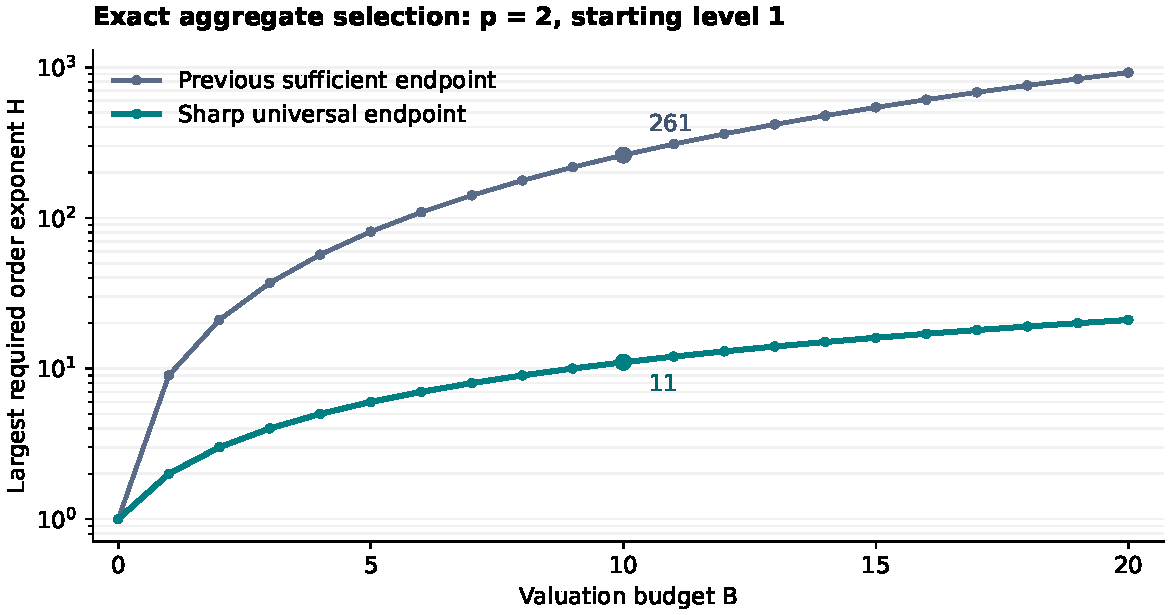
\includegraphics[width=.88\textwidth]{figures/order_bounds.pdf}
\caption{Endpoint comparison for \(p=2,h_0=1\). The vertical axis is logarithmic. The new endpoint is the exact universal threshold, while the predecessor supplied a conservative sufficient bound.}
\label{fig:bounds}
\end{figure}

At \(h_0=1\), the sharp answer simplifies to \(H_*=1+\lfloor B\rfloor\) for every prime. For an integer \(N\ge1\), the polynomial
\[
 g_N(T)=\prod_{h=1}^N\Phi_{p^h}(1+T)
       =\frac{(1+T)^{p^N}-1}{T}
\]
has \(G_\rho(g_N)=N\) for \(\rho\ge1/(p-1)\) and vanishes at every \(\zeta-1\) with \(\zeta\) a nontrivial \(p\)-power root of order at most \(p^N\). This gives an especially transparent witness that level \(N+1\) can really be necessary.

\subsection{Determinant and Fitting applications}
Let \(M_i(\mathbf T)\) be square matrices over bounded integral power series, and assume \(F_i=\det M_i\) is nonzero. If
\[
 \sum_iG_\rho(F_i)\le B,
\]
Corollary~\ref{cor:packets} gives a common torsion tuple at which all matrices are nonsingular and
\[
 \sum_i v(\det M_i(\mathbf z))\le\sum_iG_\rho(F_i).
 \tag{D}
\]
Thus the exact valuation of a product of denominator determinants can be kept within the original budget, with the optimal universal order ceiling.

If the data and the chosen torsion points lie in a finite extension \(L/\Qp\), Smith normal form gives
\[
 v_p(\det M_i(\mathbf z))
 =\frac{\operatorname{length}_{\Ocal_L}
             \operatorname{coker}M_i(\mathbf z)}
        {e(L/\Qp)}.
\]
Equation (D) therefore controls the sum of normalized finite colengths. Rectangular presentations can be treated by selecting nonzero minors, but the arithmetic presentation and its witness minors must first be supplied. The selection theorem does not construct them.

The source's denominator bookkeeping often aggregates losses, so this is a plausible place to use the stronger endpoint. Some source arguments require separate inequalities for each Selmer datum. The aggregate theorem alone is insufficient there, as the preceding counterexample proves. Replacing the source selector globally would require checking the actual objective at each call site.

\subsection{Several powers of the same parameter}
A standard product construction handles a finite list of powers, with a changed radius and budget. Suppose the integral series \(F_i\) have witness points of radius at least \(\rho\), with total valuation at most \(B\). For \(1\le j\le m\), consider
\[
 F_i\bigl((1+T_1)^j-1,\ldots,(1+T_s)^j-1\bigr).
\]
Each transformed series has a witness of coordinate valuations at least \(\rho/m\) and value equal to the original witness value. To see this, solve
\((1+y)^j=1+x\): its \(j\) roots are integral, and their valuations sum to \(v(x)\), so one has valuation at least \(v(x)/j\); if \(x=0\), take \(y=0\).

Choose \(h'_0\) with \(r_{h'_0}\le\rho/m\). Applying the sharp packet theorem with budget \(mB\) gives one tuple, of exponents at most
\[
 h'_0+\floor{p^{h'_0-1}mB},
\]
such that
\[
 \sum_{i,j}v\bigl(F_i(\zeta_1^j-1,\ldots,\zeta_s^j-1)\bigr)\le mB.
\]
The construction itself was already present in the prior exact report; the improvement here is the optimal underlying aggregate endpoint.

\subsection{Relation to existing local analysis}
The result should be compared with several established but different statements.

Bhargava's \(P\)-ordering framework organizes ultrametric interpolation and integer-valued polynomials \cite{bhargava}. The least-occupied residue branch in the proof is part of that general circle of ideas. Schefer studies quantitative \(p\)-adic Galois equidistribution of torsion points for logarithmic polynomial test functions \cite{schefer}. Those results concern averages and multiplicative independence, whereas this theorem solves an exact finite-grid worst-case problem.

Kriz--Nordentoft develop maximum-modulus principles in horizontal Iwasawa algebras and apply finite-order specialization to central-value nonvanishing \cite{kn}. This shows why a local selector is a useful arithmetic ingredient. It does not identify the present torsion-order ceiling with a global conductor ceiling: the relation between order, conductor, and admissible local behavior requires additional arithmetic information.

Serban's torsion-rigidity theorems include Lubin--Tate formal groups \cite{serban}. Our corollary concerns the sharp quantitative cost of finding one evaluation satisfying a fixed aggregate comparison; it does not strengthen the structural classification of torsion zero sets. We have established a strict improvement over the inspected ProveIt bound, but do not claim that the exact formula has never appeared elsewhere in the literature.


% Standalone section fragment; theorem environments supplied by parent manuscript.
\section{A cancellation-resistant tensor detector for icosahedral fields}
\label{sec:artin}

This section supplies a separate transfer interface. It does not improve the
smallest detector already in the incoming corpus: the $q=4$ case of the prior
$\mathrm{PSL}_2(q)$ report already has a degree-$16$ detector. The additional calculation
here is the exact first tensor power of a specified three-dimensional
representation for which proper-subgroup information alone certifies
holomorphy and detects every Dedekind zero, together with an optimal
multiplicity certificate. No literature-priority claim is made for these
finite-character identities.

\subsection{The general tensor construction}
Let $E/K$ be finite Galois with group $G$. At a point $s_0\ne1$, put
\[
 n_\psi=\operatorname{ord}_{s_0}L(s,\psi,E/K),\qquad
 \Theta=\sum_{\psi\in\operatorname{Irr}(G)}n_\psi\psi,\qquad
 d=\Theta(1)=\operatorname{ord}_{s_0}\zeta_E.
\]
The orders exist by Brauer's meromorphic continuation theorem; poles have
negative order. Classical Artin formalism gives
\[
 \langle\operatorname{Res}_C\Theta,\lambda\rangle
 =\operatorname{ord}_{s_0}L(s,\lambda,E/E^C)
 \quad(C\le G,\ \lambda\in\operatorname{Irr}(C)).
\]
When $C$ is cyclic the right side is nonnegative: its factors are finite-order
Hecke functions, with the sole possible pole at $1$. Hence
$\operatorname{Res}_C\Theta$ is a genuine character, $d\ge0$, and
$|\Theta(g)|\le d$ for every $g\in G$. Moreover $d=0$ forces $\Theta=0$.
These are classical Heilbronn-character facts, not consequences of the
proposed RH proof; see Foote--Ginsberg--Murty and Gun--Hazra--Sahu \cite{heilbronn,gun}.

Assume $G$ is nontrivial; the trivial case is immediate.
Let $\rho$ be a faithful complex representation of dimension $r$, and set
$\tau=1\oplus\rho$, $D=r+1$. Its character has
$|\chi_\tau(g)|<D$ for $g\ne1$: equality in the triangle inequality would
force every eigenvalue, including the distinguished eigenvalue $1$, to be
$1$, contradicting faithfulness. Define
\[
 F_m(g)=|\chi_\tau(g)|^{2m},\quad
 q=\max_{g\ne1}\frac{|\chi_\tau(g)|^2}{D^2}<1,
 \quad
 \kappa_m=\frac{F_m(1)-\sum_{g\ne1}F_m(g)}{|G|}.
\]
Here $F_m$ is the genuine character of
$(\tau\otimes\overline\tau)^{\otimes m}$ and is nonnegative pointwise.
If $(|G|-1)q^m<1$, then $\kappa_m>0$ and
\begin{equation}\label{eq:generic-tensor-domination}
 \kappa_m d\le\operatorname{ord}_{s_0}L(s,F_m,E/K)
 \le\langle F_m,1\rangle d.
\end{equation}
Indeed the inner product with $\Theta$ is real, its identity contribution is
$F_m(1)d/|G|$, and all other terms have absolute value at most
$F_m(g)d/|G|$. The upper bound follows by summing the same pointwise bound.
Consequently $L(s,F_m)$ is holomorphic away from $1$ and has precisely the
same zero support as $\zeta_E$ away from $1$. Its pole order at $1$ is
$\langle F_m,1\rangle$. This establishes holomorphy for an aggregate tensor
representation, not for the individual constituents of $\rho$.

For an explicit group-only sufficient exponent, if $e$ is the exponent of
$G$ then
\[
 q\le1-\frac{4\sin^2(\pi/e)}{D^2}.
\]
To prove this, diagonalize $\rho(g)$ unitarily. At least one eigenvalue
$\lambda\ne1$ is an $e$th root of unity, and
$D^2-|\chi_\tau(g)|^2$ is the sum of the squared pairwise distances among
all $D$ eigenvalues. The pair $1,\lambda$ contributes at least
$4\sin^2(\pi/e)$. This bound is deliberately crude. The character-table
certificate below is much sharper. Tensor generation itself is classical;
compare the Burnside--Brauer discussion in Steinberg \cite{steinberg}.

\subsection{An exact fourth-tensor certificate for \texorpdfstring{$A_5$}{A5}}
Write $\chi,\chi',\eta,\nu$ for the irreducible characters of degrees
$3,3,4,5$. Let $\phi=(1+\sqrt5)/2$, $\phi'=(1-\sqrt5)/2$. The table is
\[
\begin{array}{c|rrrrr}
 &1&2A&3A&5A&5B\\\hline
\text{class size}&1&15&20&12&12\\
1&1&1&1&1&1\\
\chi&3&-1&0&\phi&\phi'\\
\chi'&3&-1&0&\phi'&\phi\\
\eta&4&0&1&-1&-1\\
\nu&5&1&-1&0&0
\end{array}
\]
Let $D_5$ denote a dihedral subgroup of order $10$, with nontrivial sign
character $\epsilon$ trivial on its rotations. Choose $C_5\le D_5$ and a
nontrivial character $\lambda$ corresponding to the eigenvalues of $\chi$.
Let $\omega$ be either nontrivial character of $A_4/V_4$. Frobenius
reciprocity, or the explicit induction calculation supplied with the
archive, gives
\[
 A=\operatorname{Ind}_{D_5}^{A_5}\epsilon=\chi+\chi',\qquad
 B=\operatorname{Ind}_{C_5}^{A_5}\lambda=\chi+\eta+\nu,\qquad
 C=\operatorname{Ind}_{A_4}^{A_5}\omega=\nu.
\]
The tensor powers decompose as
\[
 \chi^2=1+\chi+\nu,\qquad
 \chi^3=1+3\chi+\chi'+\eta+2\nu,\qquad
 F=\chi^4=3+6\chi+3\chi'+4\eta+7\nu.
\]
The decisive positive identity is
\begin{equation}\label{eq:a5-fourth-certificate}
 \boxed{\ 4F=\operatorname{Reg}_{A_5}+11\cdot1+9A+12B+11C.\ }
\end{equation}
All coefficients on the right are nonnegative. For every $A_5$ extension
$E/\mathbb Q$, Artin formalism therefore gives the exact meromorphic identity
\begin{equation}\label{eq:a5-artin-product}
 L(s,F)^4=\zeta_E(s)\zeta_{\mathbb Q}(s)^{11}
 L(s,\epsilon,E/E^{D_5})^9
 L(s,\lambda,E/E^{C_5})^{12}
 L(s,\omega,E/E^{A_4})^{11}.
\end{equation}
The three displayed nontrivial one-dimensional factors are entire Hecke
functions and are nonzero at $s=1$. The right-hand side therefore has
pole order $12$ there. Since $L(s,F)$ is already meromorphic, its fourth power being
holomorphic away from $1$ implies that it too is holomorphic there.
It has pole order $3$ at $1$, the multiplicity of the trivial character.

At any $s_0\ne1$, set $e_F=\operatorname{ord}_{s_0}L(s,F)$ and
$d=\operatorname{ord}_{s_0}\zeta_E$. Equation
\eqref{eq:a5-artin-product} proves $e_F\ge d/4$.
Since $F(g)=\chi(g)^4\ge0$ and $|\Theta(g)|\le d$,
\[
 e_F=\frac1{60}\sum_gF(g)\overline{\Theta(g)}
 \le\frac d{60}\sum_gF(g)=3d.
\]
Thus
\begin{equation}\label{eq:a5-multiplicities}
 \boxed{\quad d/4\le e_F\le3d.\quad}
\end{equation}
This proves identical zero support, even when individual Artin factors
might have poles. It is stronger than merely observing that every
irreducible occurs in $F$; positive constituent multiplicities by
 themselves do not prevent cancellation of meromorphic orders.

\subsection{Exact scope of the optimality statement}
Consider the integral virtual character
\[
 \Theta_*=-\chi+\chi'+\eta.
\]
Its degree is $4$, and its restrictions to representatives of all three
maximal-subgroup types are genuine:
\[
\begin{array}{c|l}
 A_4&1+\text{the three-dimensional irreducible}\\
 D_5&2\cdot\text{one two-dimensional irreducible}\\
 S_3&1+\operatorname{sgn}+\text{the two-dimensional irreducible}.
\end{array}
\]
Each of these maximal subgroups is monomial: its irreducible characters
are induced from linear characters, so Artin--Hecke theory really does
impose these nonnegative restriction orders at an arithmetic point.
Every proper subgroup is contained in one of these maximal subgroups.
The included permutation enumeration verifies the $59$ subgroups of $A_5$
and its maximal subgroup counts: ten of order $6$, six of order $10$, and
five of order $12$. Hence $\Theta_*$ satisfies all necessary
proper-subgroup holomorphy constraints, including every cyclic restriction.
However
\[
 \langle\chi^j,\Theta_*\rangle=-1\ (j=1,2,3),\qquad
 \langle\chi^4,\Theta_*\rangle=1.
\]
Therefore the first three tensor powers cannot be certified by those
constraints, and no inequality $d\le k e_F$ valid throughout that cone can
have $k<4$. The identity \eqref{eq:a5-fourth-certificate} attains $k=4$.
This proves optimality for the algebraic cone of necessary character
conditions. It does not assert that an actual zero of any number field
realizes $\Theta_*$, nor that the first three tensor functions have poles.

For a complete small cone computation, write
$\Theta=n_0\cdot1+x\chi+y\chi'+z\eta+w\nu$ and suppose $n_0=0$.
The genuine restrictions to $A_4,D_5,S_3$ are equivalent to
\[
 z\ge0,\quad w\ge0,\quad x+y\ge0,\quad x+z+w\ge0,\quad y+z+w\ge0.
\]
Its six extreme rays in coordinates $(x,y,z,w)$ are
\[
 (1,0,0,0),\ (0,1,0,0),\ (-1,1,1,0),\ (1,-1,1,0),\
 (-1,1,0,1),\ (1,-1,0,1).
\]
To see completeness, put $s=x+y\ge0$ and
$t=(x+z+w)/(s+2z+2w)\in[0,1]$ for a nonzero vector. The vector is the
convex combination, with coefficients $t,1-t$, of
$s(1,0,0,0)+z(1,-1,1,0)+w(1,-1,0,1)$ and
$s(0,1,0,0)+z(-1,1,1,0)+w(-1,1,0,1)$.
The ratios $e_F/d$ on these rays are respectively
$2,1,1/4,7/4,4/5,2$. Thus the exact bounds in this cone are
$d/4\le e_F\le2d$. Under ordinary RH, they apply throughout
$1/2<\Re s_0<1$.

The prior degree-$16$ detector is $F_0=1+\chi+\chi'+\eta+\nu$,
with class values $(16,0,1,1,1)$ \cite{pslprior}. It can also be written
$1+\operatorname{Ind}_{V_4}^{A_5}\lambda_0$ for a nontrivial linear
character $\lambda_0$ of $V_4$. This is a more economical detector when
degree is the objective; it was already present in the inspected corpus.

For comparison, the crude pointwise dominance test fails for $\chi^4$:
its identity value is $81$, while its nonidentity sum is
$15+12(\phi^4+\phi'^4)=99$. It first succeeds among the even powers at
$\chi^6$, where $729>15+12(\phi^6+\phi'^6)=231$.
The proper-subgroup certificate therefore removes one tensor-square
amplification step; it does not improve the prior degree-$16$ detector.

\subsection{The analytic estimate still needed}
For a ramified prime, let $I$ be inertia and let $g$ be a Frobenius lift in
the decomposition group. Averaging the inertia projector gives
\[
 \operatorname{tr}\bigl(g^k\mid(\rho^{\otimes4})^I\bigr)
 =\frac1{|I|}\sum_{h\in I}\chi(g^kh)^4\ge0.
\]
Consequently the coefficients $b(p^k)$ of $D_F=-L'/L(s,F)$ are real,
nonnegative, and at most $81\log p$, including ramified primes. Let
\[
 D_F(s)=\frac3{s-1}+a_0+O(s-1)
\]
and define
\[
 T_F(x)=\sum_{n\le x}b(n)(x/n-1)-3x\log x-(a_0-3)x.
\]
For $\Re s>1$, direct integration gives
\[
 \int_1^\infty T_F(x)x^{-s-1}\,dx
 =\frac{D_F(s)}{s(s-1)}-\frac3{(s-1)^2}-\frac{a_0-3}{s-1}.
\]
The singularity at $1$ cancels. A zero $\rho$ of $L(s,F)$ contributes
residue $e_F/[\rho(1-\rho)]$, strictly positive for a real zero
$0<\rho<1$. Thus the same one-sided Mellin--Landau principle used in the
source would imply Dedekind RH for $E$ from
\[
 T_F(x)\le C_{E,\varepsilon}x^{1/2+\varepsilon}
 \quad\text{for every }\varepsilon>0\text{ and all sufficiently large }x.
\]
No such arithmetic bound is established here. The new burden is to build
short and sufficiently spanning integral sections whose long-vector
estimate encodes this tensor trace, with compatible twist and
ramification bounds. Character identities and holomorphy alone do not
supply that construction. In particular, this section does not solve
individual Artin holomorphy or establish a new case of Dedekind RH.

\section{The remaining global question, stated as an exact estimate}
\label{sec:targets}

\subsection{A complete analytic implication}
For clarity, we prove the one-sided analytic implication used in the previous section. This is a form of Landau's positivity principle, the same mechanism isolated in the Lean source.

\begin{lemma}[One-sided Mellin exclusion]
\label{lem:mellin}
Let \(T:[1,\infty)\to\mathbf R\) be locally integrable and of polynomial growth. Suppose its Mellin transform
\[
 M(s)=\int_1^\infty T(x)x^{-s-1}\,dx
\]
continues meromorphically to \(\Rea s>\theta\), with only simple poles, and every real pole in that half-plane has strictly positive residue. If
\(T(x)\le Cx^\theta\) eventually, then \(M\) has no pole in \(\Rea s>\theta\).
\end{lemma}

\begin{proof}
For a sufficiently large \(X\), the function \(f(x)=Cx^\theta-T(x)\) is nonnegative on \([X,\infty)\). Its Mellin transform is initially
\[
 Q(s)=\frac{CX^{\theta-s}}{s-\theta}
       -M(s)+\int_1^X T(x)x^{-s-1}\,dx.
\]
The finite integral is entire. Let \(\sigma_c\) be the abscissa of convergence of the nonnegative integral defining \(Q\). Polynomial growth makes it finite above; it may be \(-\infty\).

The Landau fact used here is that a nonnegative Mellin integral with finite abscissa has a singularity at the real point \(\sigma_c\). Briefly, if the transform were holomorphic there, its Taylor expansion from a real point to the right, together with nonnegative moments and monotone convergence, would force convergence slightly to the left of the abscissa, a contradiction.

If \(\sigma_c>\theta\), the displayed meromorphic expression makes that singularity a simple pole with residue equal to the negative of the corresponding residue of \(M\). It is therefore negative. But \(Q(\sigma)\ge0\) for real \(\sigma>\sigma_c\); a negative simple-pole residue would make \(Q(\sigma)\to-\infty\) as \(\sigma\downarrow\sigma_c\), which is impossible. If \(M\) has no real pole there, there is no singularity at all, giving the other contradiction. Hence \(\sigma_c\le\theta\). Absolute convergence then makes \(Q\), and thus \(M\), holomorphic in \(\Rea s>\theta\).
\end{proof}

\begin{theorem}[A concrete nonabelian RH target]
\label{thm:a5target}
Let \(E/\mathbf Q\) be Galois with group \(A_5\), and let \(F=\chi^4\) and \(T_F\) be as in Section~\ref{sec:artin}. Suppose that, for every \(\varepsilon>0\),
\[
 T_F(x)\le C_{E,\varepsilon}x^{1/2+\varepsilon}
 \qquad\text{for all sufficiently large }x.
 \tag{A5}
\]
Then every nontrivial zero of \(\zeta_E\) has real part \(1/2\). Moreover, every individual Artin factor has neither a zero nor a pole off that line inside the critical strip.
\end{theorem}

\begin{proof}
The prime-power coefficient bound gives polynomial growth and local integrability of \(T_F\). Its Mellin transform was computed exactly in the preceding section. The point \(s=1\) is removable. In \(\Rea s>0\), its other poles are simple and occur at zeros of \(L(s,F)\); their residues are
\[
 \frac{\ord_\alpha L(s,F)}{\alpha(1-\alpha)}.
\]
For real \(0<\alpha<1\) these are positive. There are no zeros for real part greater than or equal to \(1\), apart from the already removed pole at \(1\); this follows from the Artin--Hecke product identity and the classical zero-free boundary for the factors.

For each \(1/2<\theta<1\), condition (A5) and Lemma~\ref{lem:mellin} exclude zeros of \(L(s,F)\) with real part greater than \(\theta\). The multiplicity comparison \(d/4\le e_F\) excludes zeros of \(\zeta_E\) there. Letting \(\theta\downarrow1/2\), and using the functional equation of \(\zeta_E\), proves its RH.

At an off-line point in the strip, \(d=\ord\zeta_E=0\). The cyclic-restriction inequality \(|\Theta(g)|\le d\) forces the entire Heilbronn character to be zero, so all the individual Artin orders vanish.
\end{proof}

The last assertion permits possible individual Artin poles on the critical line. It does not prove the Artin holomorphy conjecture. The hypothesis (A5) is the exact missing arithmetic statement; this report does not establish it.

\subsection{Why this is a method transfer, and where it stops}
The fourth-tensor construction supplies a nonnegative prime statistic, meromorphic continuation, unconditional holomorphy of the aggregate, and a residue dictionary without cancellation. Those are enough for the analytic endgame. They do not build the arithmetic object whose determinant comparison proves (A5).

A successful adaptation of the source would still have to construct integral sections or forms for this tensor statistic; show that the short sections span almost all the required space; prove a matching lower covolume bound; control ramification and congruence denominators; and keep every loss within the square-root scale. Tensor multiplication of characters by itself proves none of those estimates.

The general faithful-tensor theorem is useful when a geometric construction naturally produces tensor powers of a representation. It supplies a finite, explicit amplification threshold. The sharp \(A_5\) certificate reduces that threshold from a sixth-power pointwise test to the fourth power. It is not the best choice if the only optimization objective is detector degree: the prior degree-16 construction remains smaller.

\subsection{Assessment of candidate problems}
\begin{center}
\small
\begin{tabularx}{\textwidth}{@{}p{.25\textwidth}XX@{}}
\toprule
Question & Progress actually supplied & Missing input or obstruction\\
\midrule
Optimal exact torsion specialization & Solved for the fixed aggregate objective, including sharpness and bounded series & Separate exact individual constraints are a different and obstructed objective.\\
Lubin--Tate specialization & Exact same minimax theorem with residue cardinality \(q\) & No global conductor or density conclusion follows from local order alone.\\
Nonabelian Dedekind RH & Explicit cancellation-safe analytic criterion and tensor certificate & A new arithmetic proof of (A5).\\
Artin holomorphy & Certain aggregate tensor products are holomorphic without the conjecture & Positivity of aggregate orders does not force each constituent order to be nonnegative on the critical line.\\
Simultaneous finite-order nonvanishing & A sharp local specialization budget for nonzero analytic packets & Integral interpolation, nonzero witnesses, admissible character realization, and conductor counting.\\
BSD or Selmer vanishing & Better aggregate determinant specialization may reduce a local search & Source hypotheses require finite conjugate-dual terms; the existing duality obstruction survives.\\
Vandiver or cyclotomic vanishing & The source supplies finite-level length bounds & A finite positive bound is not zero, and the required comparison with the target group must be proved.\\
\bottomrule
\end{tabularx}
\end{center}

For the Selmer direction, the source's \path{SelmerData.lean} explicitly assumes a finite global congruence term, finite local terms, residual spanning conditions, and an inertial scalar condition. Its general twisting theorem gives a bound of the form \(\beta_T+\varepsilon\). The rational conjugate-duality obstruction established in the preceding report is unaffected by anticyclotomic twisting \cite{structuralprior}. An improved torsion ceiling cannot make an infinite \(\beta_T\) finite.

For the cyclotomic direction, \path{Lib/Cyclotomic/OddSha.lean} bounds particular finite-level cocycle modules by valuations of an explicitly bounded nonzero integer. Even after making the comparison with a conventional cohomology group, one still needs an argument that the relevant valuation vanishes. No such argument is supplied here.

\subsection{Recommended mathematical continuation}
The best concrete next step is to formalize the sharp shell theorem and use it at source call sites whose loss is genuinely aggregate. Its hypotheses are local and its proof is finite enough to be separated from the rest of the RH development. The included formalization plan lists the required lemmas without pretending they have already been checked in Lean.

For a global extension, the decisive experiment is a construction of the upper and lower determinant estimates for one nonabelian test family, with every rank and denominator loss written out. Another character identity alone would add less than resolving even one of those arithmetic estimates. The \(A_5\) tensor formula gives a fully specified statistic against which such a construction can be tested.


\section{Verification, provenance, and reproducibility}
\label{sec:verification}

\subsection{Independent mathematical checks}
The report was prepared with AI assistance. The independent reconstructions and reviews in this archive were performed by separate collaborating agents; they are not external journal refereeing.

The torsion proof was independently reconstructed and reviewed, including:
arbitrary \(\Cp\)-roots; repeated roots; the case \(p=2,h_0=1\); integer budget boundaries; off-shell roots; nonattained coefficient infima; arbitrary finite dimension; bounded-series truncation; aggregate packets; and the Lubin--Tate normalization. The complete review is included.

The calculations supplement the proofs. They use exact integer, rational, or quadratic-field arithmetic and do not rely on floating-point estimates.

\begin{center}
\small
\begin{tabularx}{\textwidth}{@{}p{.34\textwidth}X@{}}
\toprule
Check & Scope and observed result\\
\midrule
Aggregate recurrence & 800 greedy shell recurrences and 800 floor identities: PASS.\\
Boundary thresholds & 1,440 rational budget cases, including equality: PASS.\\
Sharp constructions & 55 constructions, 22,473 primitive evaluation points: PASS.\\
Independent shell minimax & All 6,974 marked multisets in seven small shells and 27 budget cases: PASS.\\
\(A_5\) certificate & Exact character arithmetic in \(\mathbf Q(\sqrt5)\), actual subgroup induction, all 59 subgroups, maximal restrictions, and six-ray inequalities: PASS.\\
Source audit & Both editions scanned; file hashes and file-level import closure recorded. No independent kernel replay.\\
Prior-source provenance & All 31 archive lengths and Git blob hashes matched the pinned directory.\\
\bottomrule
\end{tabularx}
\end{center}

\subsection{Archive contents}
\begin{itemize}
\item \path{report.tex}, \path{report.pdf}, and \path{sections/}: complete manuscript and sources.
\item \path{code/verify_aggregate_minimax.py}: shell recurrence, equality, threshold, and extremizer checks.
\item \path{code/verify_shell_minimax_exhaustive.py}: an independent exhaustive maximin computation over small marked multisets.
\item \path{code/verify_a5_tensor.py}: exact character certificate and subgroup enumeration.
\item \path{code/make_figures.py}: exact bound table and the comparison plot.
\item \path{code/scan_source.py}: reproducible source inventory and lexical audit; requires the frozen upstream checkout.
\item \path{data/}: exact verification results and bound data.
\item \path{evidence/}: source audit, prior-corpus comparison, immutable source manifest, and independent proof review.
\item \path{formalization/plan.md}: a proposed Lean decomposition and the precise unformalized boundaries.
\item \path{build.sh}, \path{README.md}, and \path{SHA256SUMS}: reproduction instructions and archive integrity.
\end{itemize}

\subsection{Reproduction}
From the extracted directory, run:
\begin{lstlisting}
python3 code/verify_aggregate_minimax.py
python3 code/verify_shell_minimax_exhaustive.py
python3 code/verify_a5_tensor.py
python3 code/make_figures.py
bash build.sh
\end{lstlisting}
The three proof-check scripts use the Python standard library. Plotting additionally uses Matplotlib. PDF compilation uses a standard LaTeX installation and \texttt{latexmk}.

The scripts' existing exact assertions are the main reproducible checks. JSON files record the observed outputs. A supplied script is not a formal proof in Lean, and the manuscript makes no such claim.

To reproduce the upstream Lean theorem checks separately, obtain the pinned source and follow its README:
\begin{lstlisting}
cd grh
lake exe cache get
lake build
lake env lean scripts/PrintAxioms.lean
\end{lstlisting}
The upstream build was not run here. No GitHub branch, issue, pull request, or repository file was modified.

\subsection{Interpretation of the result}
The sharp torsion formula is a completed mathematical theorem, with an explicit optimality example, and improves the same objective studied in an inspected predecessor. The tensor identities are complete finite-character statements with a rigorous analytic interpretation. The new nonabelian prime-sum estimate remains a research target. These categories should remain separate when incorporating the report into ProveIt.


\begin{thebibliography}{99}
\addcontentsline{toc}{section}{References}
\bibitem{grh}
L. Sernau and contributors.
\emph{GRH for Dirichlet \(L\)-functions, in Lean 4}.
Frozen source commit \texttt{72fead102f663d5c7a407964a13dc0cf9d977207}, 25 November 2026.
\url{https://github.com/lsernau/grh-lean/tree/72fead102f663d5c7a407964a13dc0cf9d977207}.
The original repository carries Apache-2.0 licensing and attribution to Anthropic, PBC.
\bibitem{corpus}
ProveIt incoming research corpus.
31 ZIP archives at commit \texttt{274841c1cb137aafbb60ab5f519c51fd42eee98e}.
\url{https://github.com/VladimirReshetnikov/ProveIt/tree/274841c1cb137aafbb60ab5f519c51fd42eee98e/docs/incoming}.
Exact filenames, Git blob identifiers, byte lengths, and SHA-256 hashes are recorded in the accompanying evidence files.
\bibitem{exactprior}
ProveIt research report.
\emph{Exact torsion transfer}, 25 November 2026.
Archive \path{grh_exact_torsion_transfer_2026-11-25.zip} in \cite{corpus};
especially \path{sections/exact_torsion.tex}.
\prior{grh_exact_torsion_transfer_2026-11-25.zip}{Pinned archive}.
\bibitem{shellprior}
ProveIt research report.
\emph{Torsion and zero data}, 25 November 2026.
Archive \path{grh-torsion-and-zero-data.zip} in \cite{corpus};
especially the exact one-shell and positive-part minimax arguments.
\prior{grh-torsion-and-zero-data.zip}{Pinned archive}.
\bibitem{samplingprior}
ProveIt research report.
\emph{Torsion and prime sampling}, 25 November 2026.
Archive \path{grh-torsion-and-prime-sampling.zip} in \cite{corpus};
especially \path{sections/torsion.tex}, \path{sections/field.tex}, and \path{sections/limits.tex}.
\prior{grh-torsion-and-prime-sampling.zip}{Pinned archive}.
\bibitem{meanprior}
ProveIt research report.
\emph{GRH method transfers}, third indexed archive, 25 November 2026.
Archive \path{grh_method_transfers_2026-11-25 (2).zip} in \cite{corpus};
\path{sections/mean_transfer.tex} and \path{sections/mean_additions.tex}.
\bibitem{pslprior}
ProveIt research report.
\emph{\(\mathrm{PSL}_2\) GRH transfer}, 25 November 2026.
Archive \path{psl2_grh_transfer.zip} in \cite{corpus}.
The \(q=4\) case contains the degree-16 \(A_5\) detector.
\prior{psl2_grh_transfer.zip}{Pinned archive}.
\bibitem{sylowprior}
ProveIt research report.
\emph{Sylow transfer}, 25 November 2026.
Archive \path{grh_sylow_transfer_2026-11-25.zip} in \cite{corpus}.
\prior{grh_sylow_transfer_2026-11-25.zip}{Pinned archive}.
\bibitem{cyclicprior}
ProveIt research report.
\emph{Cyclic-generator transfer}, 25 November 2026.
Archive \path{grh_cyclic_generator_transfer_2026-11-25.zip} in \cite{corpus}.
\prior{grh_cyclic_generator_transfer_2026-11-25.zip}{Pinned archive}.
\bibitem{structuralprior}
ProveIt research report.
\emph{Structural transfers}, 25 November 2026.
Archive \path{grh_structural_transfers_2026-11-25.zip} in \cite{corpus};
especially \path{sections/duality.tex}.
\prior{grh_structural_transfers_2026-11-25.zip}{Pinned archive}.
\bibitem{bhargava}
M. Bhargava.
On \(P\)-orderings, rings of integer-valued polynomials, and ultrametric analysis.
\emph{Journal of the American Mathematical Society} \textbf{22} (2009), 963--993.
\url{https://doi.org/10.1090/S0894-0347-09-00638-9}.
\bibitem{lt}
J. Lubin and J. Tate.
Formal complex multiplication in local fields.
\emph{Annals of Mathematics} (2) \textbf{81} (1965), 380--387.
Theorems 1 and 2(b).
\url{https://doi.org/10.2307/1970622}.
Accessible primary text:
\url{https://www.sas.rochester.edu/mth/sites/doug-ravenel/otherpapers/lubin-tate.pdf}.
\bibitem{serban}
V. Serban.
An infinitesimal \(p\)-adic multiplicative Manin--Mumford conjecture.
\emph{Journal de Theorie des Nombres de Bordeaux} \textbf{30} (2018), 393--408.
\url{https://doi.org/10.5802/jtnb.1030}.
\url{https://www.numdam.org/item/JTNB_2018__30_2_393_0/}.
\bibitem{kn}
D. Kriz and A. C. Nordentoft.
\emph{Horizontal \(p\)-adic \(L\)-functions}.
arXiv:2310.20678, version 3, consulted 25 November 2026.
In particular, Propositions 2.7 and 2.11 and Theorem 2.8.
\url{https://arxiv.org/html/2310.20678v3}.
\bibitem{schefer}
G. Schefer.
\emph{\(p\)-adic equidistribution and an application to \(S\)-units}.
arXiv:2410.24088, version 1 (2024).
\url{https://arxiv.org/html/2410.24088v1}.
\bibitem{heilbronn}
R. Foote, H. Ginsberg, and V. Kumar Murty.
Heilbronn characters.
\emph{Bulletin of the American Mathematical Society} \textbf{52} (2015), 465--496.
\url{https://doi.org/10.1090/bull/1492}.
\bibitem{gun}
S. Gun, S. Hazra, and D. Sahu.
On holomorphy and non-vanishing of Artin \(L\)-functions.
\emph{Monatshefte fur Mathematik} \textbf{206} (2025), 853--883.
\url{https://doi.org/10.1007/s00605-025-02060-7}.
\bibitem{steinberg}
B. Steinberg.
\emph{On the Burnside--Brauer--Steinberg theorem}.
arXiv:1409.7632, version 2 (2014).
\url{https://arxiv.org/abs/1409.7632}.
\end{thebibliography}


\end{document}

